% 2D Image with indices
% Author: Peter Steinbach
\documentclass[tikz]{standalone}
\usetikzlibrary{calc,trees,positioning,arrows,chains,shapes.geometric,%
    decorations.pathreplacing,decorations.pathmorphing,shapes,%
    matrix,shapes.symbols,fit}

\pgfdeclarelayer{back}
\pgfsetlayers{back,main}


\makeatletter
\tikzset{
  fitting node/.style={
    inner sep=0pt,
    fill=none,
    draw=none,
    reset transform,
    fit={(\pgf@pathminx,\pgf@pathminy) (\pgf@pathmaxx,\pgf@pathmaxy)}
  },
  reset transform/.code={\pgftransformreset}
}
\makeatother

\begin{document}
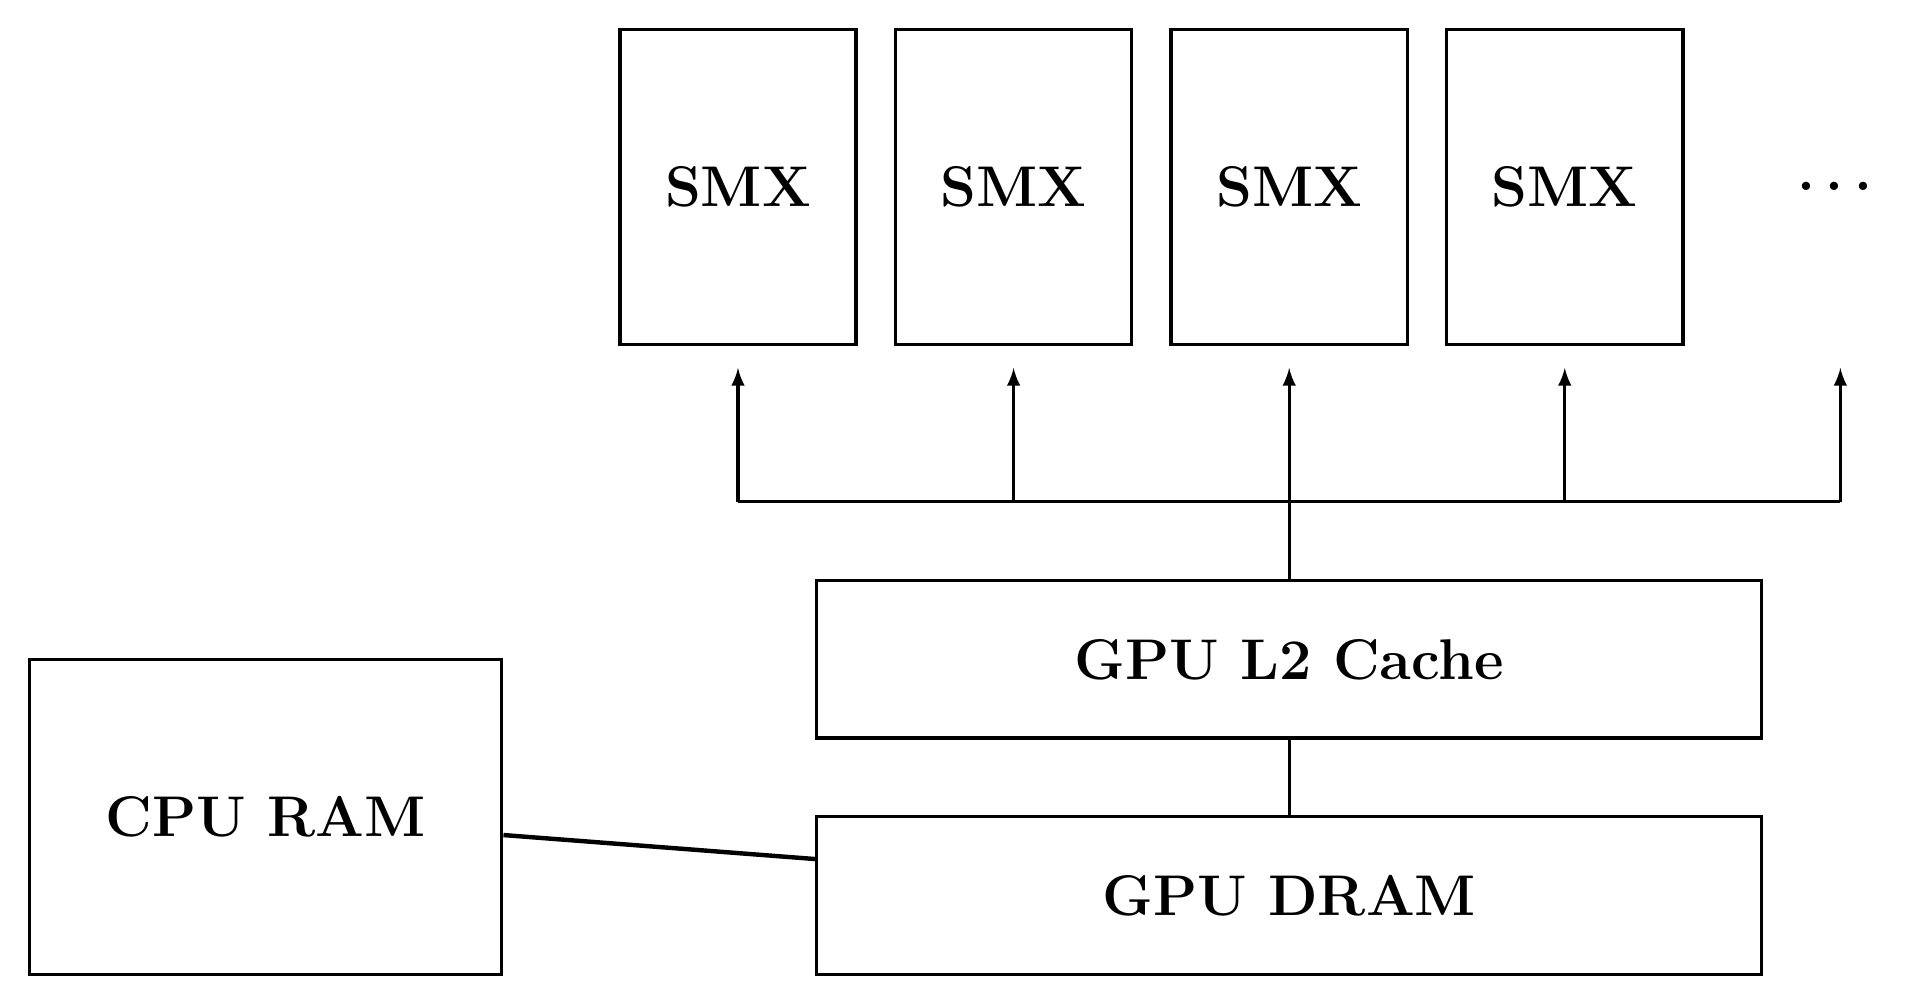
\begin{tikzpicture}[]

  \foreach \c in {0,...,3}
  {
    %\draw[-] ($(0.2,2.05)+(2.4*\c,0)$) rectangle ($(2.3,2.75)+(2.4*\c,0)$) node[fitting node] (l2_\c) {\bfseries{}L2};
    \node [very thick,draw,rectangle, minimum width=3cm, minimum height=4cm,font=\huge] at($(8,10)+(3.5*\c,0)$) {\bfseries{}SMX};
    
  }

  \foreach \i in {0,...,4}
  \draw[very thick,-latex] ($(8,6)+(3.5*\i,0)$) -- ($(8,7.7)+(3.5*\i,0)$) 
  ;
  
  \node (dots) [text=black,font=\huge] at($(8,10)+(14,0)$) {\bfseries{}\dots};

  \draw[very thick] ($(8,6)$) -- ($(8,6)+(3.5*4,0)$) ;

  \node (l2cache) [very thick,draw,rectangle, minimum width=12cm, minimum height=2cm,font=\huge] at($(8,10)+(7,-6)$) {\bfseries{}GPU L2 Cache};
  \node (dram) [very thick,draw,rectangle, minimum width=12cm, minimum height=2cm,font=\huge] at($(8,10)+(7,-9)$) {\bfseries{}GPU DRAM};

  \node (ddr4) [very thick,draw,rectangle, minimum width=6cm, minimum height=4cm,font=\huge] at($(2,10)+(0,-8)$) {\bfseries{}CPU RAM};

  \draw[ultra thick] (ddr4) -- (dram);
  \draw[very thick] (dram) -- (l2cache);
  \draw[very thick] (l2cache) -- ($(8,6)+(7,0)$);
  

\end{tikzpicture}
\end{document}
